\section{Mutation Analysis}

\begin{sloppypar}
We used the universal mutator
(\url{https://github.com/agroce/universalmutator})~\cite{regexpMut} to
mutate the code.
\end{sloppypar}

\begin{figure*}
\vspace{2mm}
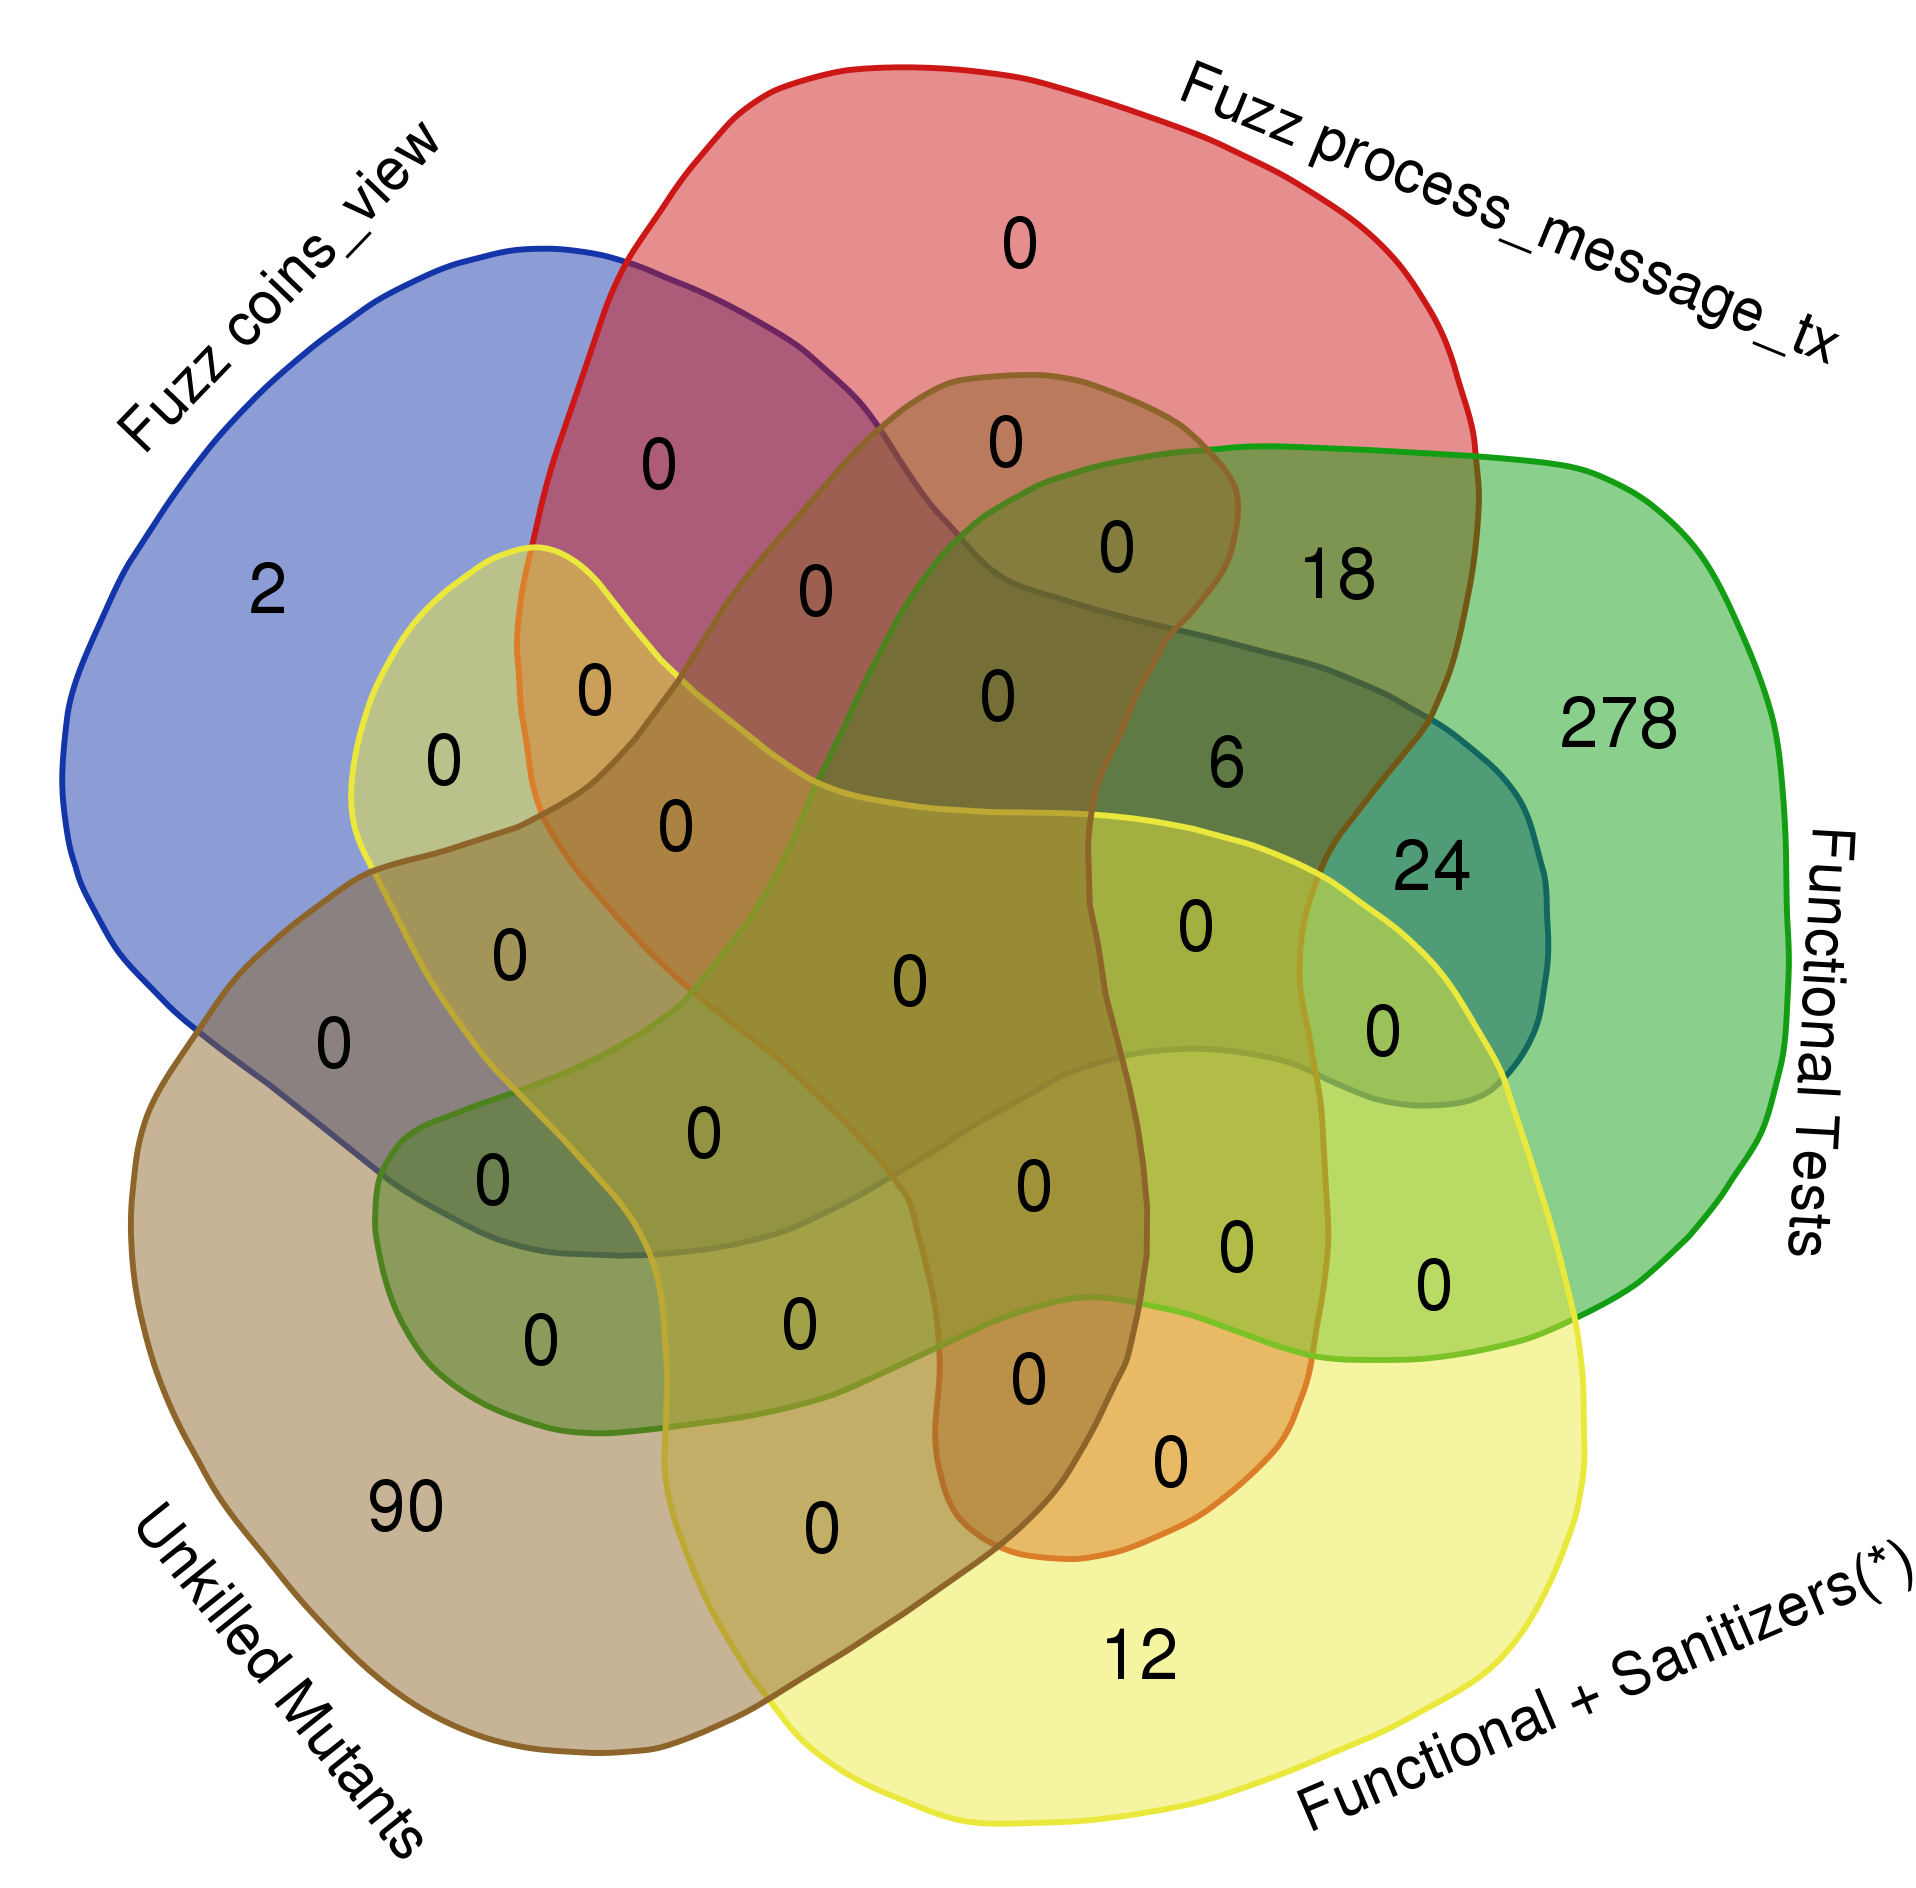
\includegraphics[width=1.9\columnwidth]{kill_pre_valgrind.png}
\caption{The Gaping Maw of Cthulhu}
\end{figure*}

\begin{figure*}
\vspace{2mm}
\centering
\begin{tabular}{llrccc}
\toprule
\bf \mr{2}{Project} & \bf \mr{2}{File Path} & \bf \mr{2}{LOC} & \mc{1}{c}{\bf Mutation} & \mc{1}{c}{\bf File}  & \mc{1}{c}{\bf Project} \\
\bf                 & \bf                   & \bf & \mc{1}{c}{\bf Score}    & \mc{1}{c}{\bf Coverage}               & \mc{1}{c}{\bf Coverage}  \\
\midrule
bitcoin & src/consensus/tx\_verify.cpp & 210 & 78.6\% & 98.7\% & 84.2\% \\
\cmidrule{2-6}
\mr{2}{go-ethereum} & core/block\_validator.go & 129 & 70.1\% & 81.0\% & 84.2\% \\
                    & signer/fourbyte/validation.go & 127 & 49.5\% & 60.0\% & 58.8\% \\
\cmidrule{2-6}
    \mr{3}{solana}   & perf/src/sigverify.rs & 1246 & ????\% & 74.48\% & \mr{3}{82.2\%} \\ 
    % & core/src/sigverify\_stage.rs &  296 & ????\% & 88.46\% & \mr{3}{82.2\%} \\  this seems to just call perf/src/sigverify
           & core/src/validator.rs & 2016 & -      & 73.29\% &        \\ % these are app.codecov.io/gh/solana-labs/solana @a6a4cfd numbers. grcov doesn't include tests, but reports coverage % as a total over lines including tests, so it's also not accurate. we'll just over approximate rather than underapproximate
           & core/src/tvu.rs       &  494 & -      & 63.12\% &       \\ 
\cmidrule{2-6}
  dogecoin & src/bitcoin-tx.cpp & 847 & 58.7\% & - & 70.1\% \\
\cmidrule{2-6}
  avalanchego & vms/platformvm/add\_subnet\_validator\_tx.go & 308 & 57.3\% & 81.0\% & 63.6\% \\
\cmidrule{2-6}
  stellar & src/historywork/VerifyTxResultsWork.cpp & 192 & 85.1\% & - & - \\
\cmidrule{2-6}
  go-algorand & ledger/eval.go & 1551 & 99.8\% & 86.0\% & 52.2\% \\
\cmidrule{2-6}
  cosmos-sdk & x/auth/ante/sigverify.go & 510 & 73.1\% & - &  - \\
\bottomrule
\end{tabular}

\caption{Comparison of Coverage and Mutation Score Across Projects}
\label{fig:comparison}
\end{figure*}

\subsection{Comparison with Other Cryptocurrency Codebases}

We use universal mutator to compare Bitcoin's testing quality with other popular cryptocurrencies. Transaction validation logic was targeted
due to this logic being very critical and having a high likelihood to cause high severity issues in the case a bug was caught. To select
our corpus, we examined the top 10 cryptocurrencies by market cap. We eliminate stable cryptocurrencies, such as USD coin,
because they do not have transaction validation logic analagous to bitcoin. For each project, we also run coverage collection
tools in order to compare code coverage. If a project does not build or have coverage, we also exclude it from our comparison.

In the end, the following projects failed to compile: Binance Coin, Polkadot, Chainlink and the following projects did not have
readily accessable coverage reports: Stellar.

In deciding what files to mutate, we select the core transaction validation logic, by filtering for files
with tx, transaction, verify, and validate. Following this, we manually inspected each matching file and select
ones that directly relate to transaction validation. The results for these experiments are displayed in figure \ref{fig:comparison}.